\subsection{GPU Accelerating \textit{k}mer Hashing} \label{methods:gpu_accelerating_kmer_hashing}
The \textit{k}mer hashing component of KAGE is responsible for reading genomic reads from FASTA, FASTQ or other file types, encoding the reads as 2-bit encoded data and finally hashing all valid \textit{k}mers from the 2-bit encoded reads.
In KAGE, the final product yielded by this component is a 64-bit unsigned integer array where each element is a 2-bit encoded 31-mer represented in the right-most 62 bits of the integer.
Since the number of valid \textit{k}mers in a typical FASTA or FASTQ from sequencing a human genome is extremely vast, the file is usually read, encoded and hashed in chunks to alleviate the required amount of memory.
Functionality for this exists in the BioNumPy Python package.
BioNumPy implements this using NumPy and some parts of npstructures, resulting in an efficient solution that relies on NumPy's fast array operations for its performance.

\subsubsection{Implementation}
The Python package BioNumPy, which provides an implementation for \textit{k}mer encoding and hashing directly in Python, is built on top of NumPy and npstructures.
We utilized the method we described in section \ref{methods:initial_testing} and used CuPy as a drop-in replacement for NumPy to add further GPU acceleration support to npstructures, and to add partial GPU support to BioNumPy.
The resulting pipeline remained the same, but with two notable differences.
\begin{compactenum}
  \item The raw byte chunk read from the FASTA files would be copied directly to the GPU.
  \item The chunk of data received on the GPU would go through the same pipeline of array operations to 2-bit encode and hash the \textit{k}mers, but on the GPU as opposed to the CPU.
\end{compactenum}

\definecolor{cpucolor}{RGB}{255,255,225}
\definecolor{gpucolor}{RGB}{225,255,255}

\begin{figure}[H]
\begin{center}
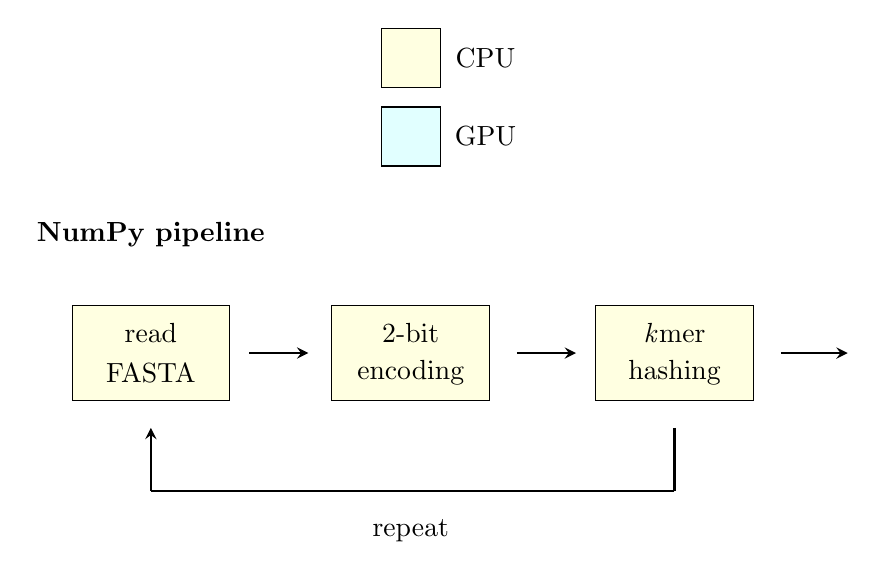
\begin{tikzpicture}
  \node at(4.25,3.75)[]{\smaller{CPU}};
  \node at(4.25,2.75)[]{\smaller{GPU}};
  \node at(3.3,3.75)[draw,minimum width=.75cm,minimum height=.75cm,fill=cpucolor]{};
  \node at(3.3,2.75)[draw,minimum width=.75cm,minimum height=.75cm,fill=gpucolor]{};
  \node at(0,1.5)[]{\smaller{\textbf{NumPy pipeline}}};
  % read fasta
  \node at(0,0)[draw,minimum width=2cm,minimum height=1.2cm,fill=cpucolor](start){};
  \node at(0,.25)[]{\smaller{read}};
  \node at(0,-.25)[]{\smaller{FASTA}};
  \draw [thick,-stealth](1.25,0) -- (2,0);
  % cpu2gpu copy
  \node at(3.3,0)[draw,minimum width=2cm,minimum height=1.2cm,fill=cpucolor]{};
  \node at(3.3,.25)[]{\smaller{2-bit}};
  \node at(3.3,-.25)[]{\smaller{encoding}};
  \draw [thick,-stealth](4.65,0) -- (5.4,0);
  % 2-bit encoding
  \node at(6.65,0)[draw,minimum width=2cm,minimum height=1.2cm,fill=cpucolor]{};
  \node at(6.65,.25)[]{\smaller{\textit{k}mer}};
  \node at(6.65,-.25)[]{\smaller{hashing}};
  \draw [thick,-stealth](8,0) -- (8.85,0);
  % arrows
  \draw [thick](6.65,-.95) -- (6.65,-1.75);
  \draw [thick](6.65,-1.75) -- (0,-1.75);
  \draw [thick,-stealth](0,-1.75) -- (0,-.95);
  \node at(3.3,-2.25)[]{\smaller{repeat}};
\end{tikzpicture}
\end{center}
\end{figure}

\begin{figure}[H]
\begin{center}
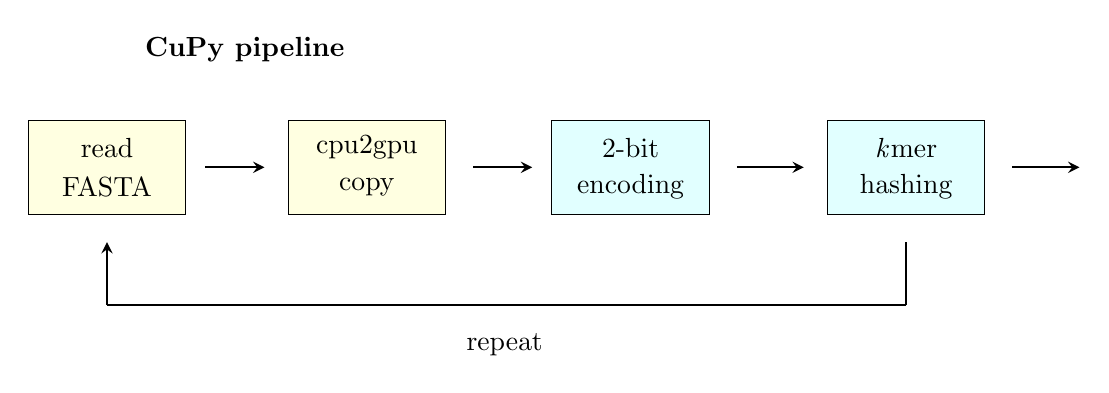
\begin{tikzpicture}
  \node at(1.75,1.5)[]{\smaller{\textbf{CuPy pipeline}}};
  % read fasta
  \node at(0,0)[draw,minimum width=2cm,minimum height=1.2cm,fill=cpucolor](start){};
  \node at(0,.25)[]{\smaller{read}};
  \node at(0,-.25)[]{\smaller{FASTA}};
  \draw [thick,-stealth](1.25,0) -- (2,0);
  % cpu2gpu copy
  \node at(3.3,0)[draw,minimum width=2cm,minimum height=1.2cm,fill=cpucolor]{};
  \node at(3.3,.25)[]{\smaller{cpu2gpu}};
  \node at(3.3,-.25)[]{\smaller{copy}};
  \draw [thick,-stealth](4.65,0) -- (5.4,0);
  % 2-bit encoding
  \node at(6.65,0)[draw,minimum width=2cm,minimum height=1.2cm,fill=gpucolor]{};
  \node at(6.65,.25)[]{\smaller{2-bit}};
  \node at(6.65,-.25)[]{\smaller{encoding}};
  \draw [thick,-stealth](8,0) -- (8.85,0);
  % kmer hashing
  \node at(10.15,0)[draw,minimum width=2cm,minimum height=1.2cm,fill=gpucolor]{};
  \node at(10.15,.25)[]{\smaller{\textit{k}mer}};
  \node at(10.15,-.25)[]{\smaller{hashing}};
  \draw [thick,-stealth](11.50,0) -- (12.35,0);
  % arrows
  \draw [thick](10.15,-.95) -- (10.15,-1.75);
  \draw [thick](10.15,-1.75) -- (0,-1.75);
  \draw [thick,-stealth](0,-1.75) -- (0,-.95);
  \node at(5.05,-2.25)[]{\smaller{repeat}};
\end{tikzpicture}
\caption{
  By using CuPy as a drop-in replacement to add GPU acceleration to KAGE's \textit{k}mer hashing step, we effectively introduced a new step in the pipeline: copying the raw text data read from the FASTA file directly to the GPU to allow for all of BioNumPy's array operations that constitute 2-bit encoding and hashing the \textit{k}mers to be performed on the GPU.
}
\label{methods:gpu_accelerating_kmer_hashing:figures:gpu_pipeline}
\end{center}
\end{figure}

Upon completing the 2-bit encoding and \textit{k}mer hashing of the chunk, the resulting \textit{k}mer array already resides in GPU memory for the counting step.
Previously, when the 2-bit encoding and \textit{k}mer hashing was performed using only the CPU, the resulting \textit{k}mer array would need to be copied to the GPU for counting when deploying the GPU accelerated \textit{k}mer counting functionality detailed in section \ref{methods:gpu_accelerating_kmer_counting}.

\subsubsection{Assessment}
Include runtime data from benchmarking the GPU accelerated 2-bit encoding and \textit{k}mer hashing component against the CPU version.
